 \part{Fourier解析}
		\chapter{Fourier級数展開}
			\section{基底関数}
				Fourier級数展開の基底関数はFourier変換やDFTのものと違って正規化されていないため、美しさに欠ける。
				\par
				$d\in\naturalNumbers,\;W_l>0\;(l=1,2,,\cdots,d),\;\bm{k}\in\integers^d$とする。
				次式で定義される、$\bm{x}\in\realSpace^d$に関する連続座標信号を、区間$\prod_{l=1}^d [-W_l,W_l]$に於ける第$\bm{k}$基底関数という。
				\[ W(\bm{k},\bm{x}) := \exp i\sum_{l=1}^d k_l\frac{x_l}{W_l}\pi \]
			
			\section{Fourier係数}
				$d\in\naturalNumbers,\;W_l>0\;(l=1,2,,\cdots,d),\;\Omega:=\prod_{l=1}^d [-W_l,W_l],\;\bm{k}\in\integers^d$とする。
				$f:\bm{x}\in\realSpace \mapsto f(\bm{x})\in\realSpace$を、第$l$座標に関して周期が$2W_l$であるような周期関数とする。
				次式で定義する、$\bm{k}$に関する離散座標信号を$f$の第$\bm{k}$Fourier係数という。
				\[ c(f,\bm{k}) := \left(\prod_{l=1}^d 2W_l\right)^{-1}\integ{\Omega}{}{\overline{W(\bm{k},\bm{x})}f(\bm{x})}{\bm{x}} \]
			
		\chapter{Fourier変換}
			\section{基底関数}
				$d\in\naturalNumbers,\;\bm{x},\bm{\omega}\in\realSpace^d$とする。
				次のものを$d$次元Fourier変換に於ける基底関数という。
				\[ W(\bm{\omega},\bm{x}) := (2\pi)^{-d/2}\exp i\bm{\omega}^\top\bm{x} \]
			
			\section{Fourier変換の定義}
				$d\in\naturalNumbers,\;\bm{\omega}\in\realSpace^d$とする。
				$f:\realSpace^d\to\complexSpace$に対して、次式で定義される、$\omega$に関する連続座標信号を$f$のFourier変換という。
				\[ \mathcal{F}(f,\bm{\omega}) := \integ{\realSpace^d}{}{\overline{W(\bm{\omega},\bm{x})}f(\bm{x})}{\bm{x}} = (2\pi)^{-d/2} \integ{\realSpace^d}{}{\exp (-i\bm{\omega}^\top\bm{x})f(\bm{x})}{\bm{x}} \]

		\chapter{離散Fourier変換(DFT)}
			\section{基底}
				$d\in\naturalNumbers,\;N_l\in\naturalNumbers\;(l=1,2,\cdots,d),\;\bm{k},\bm{n}\in\integers^d$とする。
				次式で定義される、$\bm{n}$に関する離散座標信号を$d$次元DFTの第$\bm{k}$基底ベクトルという。
				\[ W(\bm{k},\bm{n}) := \left(\prod_{l=1}^d N_l\right)^{-1/2} \exp i\left(\sum_{l=1}^d \frac{k_l n_l}{N_l}2\pi\right)\]
		
			\section{DFTの定義}
				$d\in\naturalNumbers,\;N_l\in\naturalNumbers\;(l=1,2,\cdots,d),\;\bm{k}\in\integers^d$とする。
				$f$を、定義域が$\Omega := \{0,1,\cdots,N_1-1\}\times\{0,1,\cdots,N_2-1\}\times\cdots\times\{0,1,\cdots,N_d-1\}$であるような離散座標信号$f: \Omega\to\field;\;\bm{n} = [n_1,n_2,\cdots,n_d]^\top \mapsto f(\bm{n})$とするとき、次式で定義される、$\bm{k}$に関する離散座標信号を$f$のDFTという。
				\[ \text{DFT}(f,\bm{k}) := \sum_{\bm{n}\in\Omega} \overline{W(\bm{k},\bm{n})} f(\bm{n}) \]
		
			\section{巡回畳み込みのDFTはDFTの積に比例する}
				\begin{shadebox}
					$d\in\naturalNumbers,\;N_l\in\naturalNumbers\;(l=1,2,\cdots,d),\;\bm{k}\in\integers^d$とする。
					$f,g$を、定義域が$\Omega := \{0,1,\cdots,N_1-1\}\times\{0,1,\cdots,N_2-1\}\times\cdots\times\{0,1,\cdots,N_d-1\}$であるような離散座標信号$f,g: \Omega\to\field;\;\bm{n} = [n_1,n_2,\cdots,n_d]^\top \mapsto f(\bm{n}),g(\bm{n})$とするとき、次が成り立つ。
					\[ \text{DFT}\left(\cycConv{f}{g},\bm{k}\right) = \left(\prod_{l=1}^d N_l\right)^{1/2}\text{DFT}(f,\bm{k})\text{DFT}(g,\bm{k}) \]
				\end{shadebox}
				\begin{proof}
					\quad\par
					$\bm{N} := [N_1,\cdots,N_d]^\top$とする。
					\begin{align*}
						\text{DFT}\left(\cycConv{f}{g},\bm{k}\right) &= \sum_{\bm{n}\in\Omega}\overline{W(\bm{k},\bm{n})} \left(\cycConv{f}{g}\right)(\bm{n}) = \sum_{\bm{n}\in\Omega}\overline{W(\bm{k},\bm{n})} \sum_{\bm{m}\in\Omega} f(\bm{m})g((\bm{n}-\bm{m})\%\bm{N}) \\
						&= \sum_{\bm{m}\in\Omega} f(\bm{m}) \sum_{\bm{n}\in\Omega} \overline{W(\bm{k},\bm{n})}g((\bm{n}-\bm{m})\%\bm{N}) \\
						&= \sum_{\bm{m}\in\Omega} f(\bm{m}) \sum_{\bm{n}\in\Omega} \left(\prod_{l=1}^d N_l\right)^{1/2} \overline{W(\bm{k},\bm{m})} \overline{W(\bm{k},\bm{n}-\bm{m})} g((\bm{n}-\bm{m})\%\bm{N}) \\
						&= \left(\prod_{l=1}^d N_l\right)^{1/2} \sum_{\bm{m}\in\Omega} \overline{W(\bm{k},\bm{m})}f(\bm{m}) \sum_{\bm{n}\in\Omega} \overline{W(\bm{k},(\bm{n}-\bm{m})\%\bm{N})} g((\bm{n}-\bm{m})\%\bm{N}) \\
						&= \left(\prod_{l=1}^d N_l\right)^{1/2} \sum_{\bm{m}\in\Omega} \overline{W(\bm{k},\bm{m})}f(\bm{m}) \sum_{\bm{n}\in\Omega} \overline{W(\bm{k},\bm{n})} g(\bm{n}) \\
						&= \left(\prod_{l=1}^d N_l\right)^{1/2}\text{DFT}(f,\bm{k})\text{DFT}(g,\bm{k})
					\end{align*}
				\end{proof}
		
		\chapter{サンプリング定理}
			\begin{shadebox}
				$d\in\naturalNumbers,\;W_l>0\;(l=1,2,,\cdots,d),\;\Omega:=\prod_{l=1}^d [-W_l,W_l]$とする。
				$f:\realSpace^d\to\realSpace$のFourier変換$\mathcal{F}(f,\bm{\omega})$が存在してその台が$\Omega$に含まれるとき、次式が成り立つ。
				\[ f(\bm{x}) = \sum_{\bm{n}\in\naturalNumbers}f\left(\pi\frac{n_1}{W_1},\cdots,\pi\frac{n_d}{W_d}\right)\prod_{l=1}^d\sinc W_l\left(x_l + \pi\frac{n_l}{W_l}\right) \]
				つまり$f$の各点での評価値を沢山集めて$f$を任意の精度で近似できる。
				\par
				角周波数$W_l$のかわりに周波数$F_l=W_l/(2\pi)$を使うと上式は次式になる。
				\[ f(\bm{x}) = \sum_{\bm{n}\in\naturalNumbers}f\left(\frac{n_1}{2F_1},\cdots,\frac{n_d}{2F_d}\right)\prod_{l=1}^d\sinc 2\pi F_l\left(x_l + \frac{n_l}{2F_l}\right) \]
			\end{shadebox}
			\begin{proof}
				\quad\par
				$\mathcal{F}(f,\bm{\omega})$の台が超直方体$\Omega$に含まれるから$\mathcal{F}(f,\bm{\omega})$はFourier級数展開できる。
				第$\bm{n}$Fourier係数を$c(\mathcal{F}(f),\bm{n})$とすると
				\[ \mathcal{F}(f,\bm{\omega}) = \sum_{\bm{n}\in\naturalNumbers^d} c(\mathcal{F}(f),\bm{n}) \exp i\sum_{l=1}^d n_l\frac{\omega_l}{W_l}\pi \]
				となる。$c(\mathcal{F}(f),\bm{n})$は次式で求まる。
				\begin{align*}
					c(\mathcal{F}(f),\bm{n}) &= \left(\prod_{l=1}^d 2W_l\right)^{-1} \integ{\Omega}{}{\mathcal{F}(f,\bm{\xi}) \exp (-i)\sum_{l=1}^d n_l\frac{\xi_l}{W_l}\pi}{\bm{\xi}} \\
					&= (2\pi)^{d/2} \left(\prod_{l=1}^d 2W_l\right)^{-1} (2\pi)^{-d/2} \integ{\textcolor{darkpastelgreen}{\realSpace^d}}{}{\mathcal{F}(f,\bm{\xi}) \exp i\sum_{l=1}^d \left(\frac{-n_l}{W_l}\pi\right)\xi_l}{\bm{\xi}} \\
					&= (2\pi)^{d/2} \left(\prod_{l=1}^d 2W_l\right)^{-1} \mathcal{F}^{-1}\left(\mathcal{F}(f),\frac{-\pi\bm{n}}{\bm{W}}\right) \\
					&= (2\pi)^{d/2} \left(\prod_{l=1}^d 2W_l\right)^{-1} f\left(\frac{-\pi\bm{n}}{\bm{W}}\right)
				\end{align*}
				$f$は$\mathcal{F}(f)$のFourier逆変換で次のようにして求まる。
				\begin{align*}
					f(\bm{x}) &= \mathcal{F}^{-1}\left(\mathcal{F}(f),\bm{x}\right) = (2\pi)^{-d/2} \integ{\realSpace^d}{}{\mathcal{F}(f,\bm{\omega})\exp i\bm{\omega}^\top\bm{x}}{\bm{\omega}} = (2\pi)^{-d/2} \integ{\Omega}{}{\mathcal{F}(f,\bm{\omega})\exp i\bm{\omega}^\top\bm{x}}{\bm{\omega}} \\
					&= (2\pi)^{-d/2} \integ{\Omega}{}{\sum_{\bm{n}\in\naturalNumbers^d} c(\mathcal{F}(f),\bm{n}) \left(\exp i\sum_{l=1}^d n_l\frac{\omega_l}{W_l}\pi\right) \exp i\bm{\omega}^\top\bm{x}}{\bm{\omega}} \\
					&= (2\pi)^{-d/2} \sum_{\bm{n}\in\naturalNumbers^d} \integ{\Omega}{}{c(\mathcal{F}(f),\bm{n}) \exp i \bm{\omega}^\top\left(\bm{x} + \pi\frac{\bm{n}}{\bm{W}}\right) }{\bm{\omega}} \\
					&= (2\pi)^{-d/2} \sum_{\bm{n}\in\naturalNumbers^d} \integ{\Omega}{}{(2\pi)^{d/2} \left(\prod_{l=1}^d 2W_l\right)^{-1} f\left(\frac{-\pi\bm{n}}{\bm{W}}\right) \exp i \bm{\omega}^\top\left(\bm{x} + \pi\frac{\bm{n}}{\bm{W}}\right) }{\bm{\omega}} \\
					&= \left(\prod_{l=1}^d 2W_l\right)^{-1} \sum_{\bm{n}\in\naturalNumbers^d} f\left(\frac{-\pi\bm{n}}{\bm{W}}\right) \integ{\Omega}{}{\exp i \bm{\omega}^\top\left(\bm{x} + \pi\frac{\bm{n}}{\bm{W}}\right) }{\bm{\omega}}
				\end{align*}
				ここで
				\begin{align*}
					\integ{\Omega}{}{\exp i \bm{\omega}^\top\left(\bm{x} + \pi\frac{\bm{n}}{\bm{W}}\right) }{\bm{\omega}} &= \prod_{l=1}^d \integ{-W_l}{W_l}{\exp i\left(x_l + \pi\frac{n_l}{W_l}\right)\omega_l}{\omega_l} \\
					&= \prod_{l=1}^d \frac{1}{i\left(x_l + \pi\frac{n_l}{W_l}\right)}\left[\exp i\left(x_l + \pi\frac{n_l}{W_l}\right)W_l - \exp (-i)\left(x_l + \pi\frac{n_l}{W_l}\right)W_l\right] \\
					&= \prod_{l=1}^d 2W_l \frac{\sin \left(x_l + \pi\frac{n_l}{W_l}\right)W_l}{\left(x_l + \pi\frac{n_l}{W_l}\right)W_l} = \prod_{l=1}^d 2W_l \prod_{l=1}^d \sinc W_l\left(x_l + \pi\frac{n_l}{W_l}\right)
				\end{align*}
				より、
				\begin{align*}
					f(\bm{x}) &= \sum_{\bm{n}\in\naturalNumbers^d} f\left(\frac{-\pi\bm{n}}{\bm{W}}\right) \prod_{l=1}^d 2W_l \sinc \left(x_l + \pi\frac{n_l}{W_l}\right)W_l = \sum_{\bm{n}\in\naturalNumbers^d} f\left(\frac{\pi\bm{n}}{\bm{W}}\right) \prod_{l=1}^d \sinc W_l\left(x_l - \pi\frac{n_l}{W_l}\right) \\
					&= \sum_{\bm{n}\in\naturalNumbers^d} f\left(\pi\frac{n_1}{W_1},\cdots,\pi\frac{n_d}{W_d}\right) \prod_{l=1}^d \sinc W_l\left(x_l - \pi\frac{n_l}{W_l}\right)
				\end{align*}
			\end{proof}
		\chapter{高速Fourier変換(FFT)}
			\section{長さが2のべき乗でない信号のDFTを長さが2のべき乗の信号のFFTに帰着する方法}
				$N$を$2$のべき乗でない自然数とする。
				長さ$N$の信号$x$のDFT
				\[ X(k) = \frac{1}{\sqrt{N}} \sum_{n=0}^{N-1} x(n)\exp \left(2\pi i\frac{-kn}{N}\right) \quad k=1,2,\cdots,N-1 \]
				を長さが$2$のべき乗である信号のFFTに帰着する方法を考える。
				$\forall a,b\in\mathbb{R},\;ab = \frac{a^2 + b^2 - (a-b)^2}{2}$を用いて上の式を次のように変形する。
				\begin{align*}
					\begin{aligned}
						X(k) &= \frac{1}{\sqrt{N}} \exp \left(\pi i\frac{-k^2}{N}\right) \sum_{n=0}^{N-1} x(n)\exp \left(\pi i\frac{-n^2}{N}\right) \exp \left(\pi i\frac{(k-n)^2}{N}\right) \\
						&= \frac{1}{\sqrt{N}} \exp \left(\pi i\frac{-k^2}{N}\right) \sum_{n=0}^{N-1} u(n)v(k-n) \\
						& \text{where} \quad u(n) := x(n)\exp \left(\pi i\frac{-n^2}{N}\right),\;v(n) := \exp \left(\pi i\frac{n^2}{N}\right)
					\end{aligned}
				\end{align*}
				\[ \therefore\; X(k)\sqrt{N} \exp \left(\pi i\frac{k^2}{N}\right) = (u*v)(k) \]
				$u*v$を、長さが$2$のべき乗の信号に対して使えるFFT, IFFTを用いて計算する。
				そのために長さが$2$のべき乗の信号同士の**巡回畳み込み**の中に$u*v$が部分的に現れるような状況を以下のようにして作り出す。
				\par
				$N_2 := \min\{a|\exists b\in \mathbb{N}, a = 2^b \geq 2N\}$ とする。
				長さ$N_2$の信号$u_2,v_2$を以下のように定義する。
				\[
					u_2(n) := \left\{
						\begin{aligned}
							u(n) &\quad (n \in [0,N-1]) \\
							0 &\quad (n \in [N,N_2-1])
						\end{aligned}
					\right.
				\]
				\[
					v_2(n) := \left\{
						\begin{aligned}
							v(n) &\quad (n \in [0,N-1]) \\
							0 &\quad (n\in [N,N_2-N]) \\
							v(N_2-n) &\quad (n \in [N_2-N+1,N_2-1])
						\end{aligned}
					\right.
				\]
				$u_2$は$u$の後ろに$0$を並べて長さ$N_2$に拡張した信号である。
				$v_2$は長さ$N_2$の$0$が並んだ信号の前部を$v$で塗り替え、後部を$v$の第$1\sim N-1$要素をコピーして順番を逆にしたもので塗り替えた信号である。
				下の図は$u_2,v_2$を視覚的に表現したものである。
				\begin{figure}[H]
					\centering
					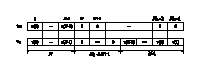
\includegraphics[keepaspectratio, scale=4]
					{parts/FourierAnalysis/imgs/FFT/arbitraryLengthFFT_to_powerOf2_FFT/u2,v2.eps}
					\caption{$u_2,v_2$の構造}
				\end{figure}
				このようにすると$u_2*v_2$の先頭$N$要素が$u*v$と一致する。
				\[ \text{FFT}(u_2*v_2) = \sqrt{N_2}\text{ FFT}(u_2) \text{ FFT}(v_2) \]
				より
				\[ \text{IFFT}(\sqrt{N_2}\text{ FFT}(u_2) \text{ FFT}(v_2)) \]
				により$u_2*v_2$を高速に計算し、結果の先頭$N$要素を切り出せば$u*v$を得る。
				得られた$u*v$の第$k$要素に$\frac{1}{\sqrt{N}} \exp \left(\pi i\frac{-k^2}{N}\right)$を掛ければ$x$のDFTが得られる。
				$v_2$のFFTや$\frac{1}{\sqrt{N}} \exp \left(\pi i\frac{-k^2}{N}\right) \;(k=0,1,\cdots,N-1)$は初回の計算結果を保存しておけば別の信号のDFTの計算で再利用できる。
